\subsection{Classificação de Cor}
Este é considerado o ``Hello World'' de SOMs. A maioria dos tutoriais publicados no
SOMs usam a classificação de cor como seu principal exemplo. Isto é para uma boa razão. Ao passar por este exemplo, o conceito de SOMs pode ser solidamente apreendido. A razão pela qual a classificação de cor é bastante fácil de entender é por causa da quantidade relativamente pequena de dados utilizados, bem como o aspecto visual dos dados.

A classificação de cores do SOM usam apenas três pesos por nó de saída e nós de entrada. Estes pesos representam a tripla (r, g, b) para a cor. Por exemplo, as cores podem ser apresentado à rede, (1,0,0) para o vermelho, (0,1,0) para o verde, etc. A meta para a rede aqui é aprender a representar todas essas cores de entrada em sua grade de duas dimensões. Com isso em mente, se azul escuro e azul claro são apresentados ao SOM, eles devem acabar ao lado do outro na grade de rede.

Para ilustrar o processo passo a passo do algoritmo de classificação da cor, o primeiro passo consiste em inicializar a rede, como mostra a figura \ref{fig:initial-node}.

\begin{figure}[ht]
\centering
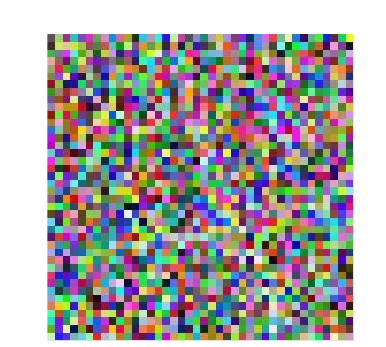
\includegraphics[width=0.7\textwidth]{imgs/initial-node.png}
\caption{Disposição inicial dos neurônios}
\label{fig:initial-node}
\end{figure}


Em seguida, temos que escolher um vetor de forma aleatória a partir dos vetores de entrada. Oito vetores de entrada são utilizados neste exemplo, que vão do vermelho para o amarelo para verde escuro. 

Posteriormente, o próximo passo é passar por cada nó e encontrar BMU (Best Matching Unit, utilizando a distância euclidiana, por exemplo). A Figura \ref{fig:bmu-node} mostra o BMU sendo selecionado na rede 4x4.

Com o BMU encontrada, o raio vizinhança deve ser calculado, como também mostrado na Figura \ref{fig:bmu-node}. Todos os nós em vermelho estão dentro do raio. 

Por último, aplica-se o aprendizado para todos esses nós. O aprendizado baseia-se na distância do neurônio em relação a entrada apresentada.

\begin{figure}[ht]
\centering
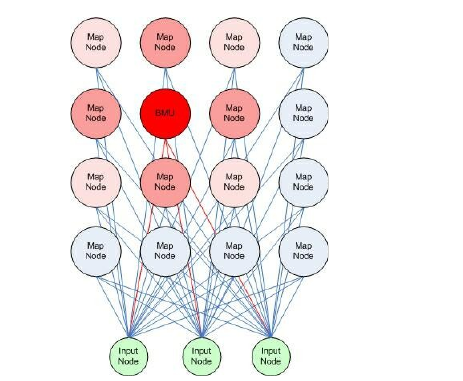
\includegraphics[width=0.7\textwidth]{imgs/node-bmu.png}
\caption{Nó vencedor}
\label{fig:bmu-node}
\end{figure}

Em seguida, um novo vetor aleatório é escolhido e todo processo se repete. A Figura \ref{fig:final-node} mostra um SOM treinado, representando todas as cores das oito entradas de cores. Observe como a cor verde fica ao lado do verde escuro e a cor vermelha está ao lado da cor laranja.

\begin{figure}[ht]
\centering
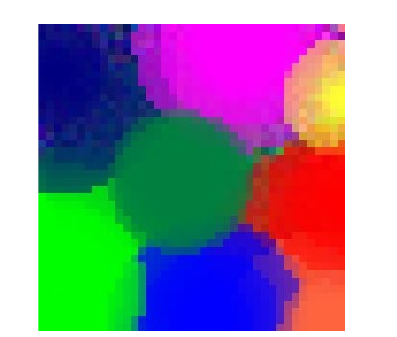
\includegraphics[width=0.5\textwidth]{imgs/final-node.png}
\caption{Estrutura do nó final}
\label{fig:final-node}
\end{figure}